\section{Introduction}
\label{sec:introduction}

Unsupervised graph domain adaptation (UGDA) transfers a node classifier from a
labeled source graph to an unlabeled target graph whose attributes and topology
may follow a different distribution~\citep{wu2020unsupervised,dai2022graph,liu2023structural}.
Recent methods address propagation mismatch, conditional structure shift,
homophily shift, and composite feature--structure shift with increasingly
specialized adaptation objectives~\citep{liu2023structural,liu2024rethinking,liu2024pairwisealignmentimprovesgraph,fang2025attribute, yang2025disentangled,pmlr-v267-fang25g,chen2026learningadaptivedistributionalignment}.
These advances primarily answer how a candidate model should be trained.
Deployment poses a distinct question: without target labels, which algorithm,
hyperparameter setting, random seed, and checkpoint should be used? This paper
studies that selection problem rather than proposing another adaptation loss.

This question is obscured when target labels are used after training to select
the best checkpoint. For example, our audit of the public ADAlign
implementation\footnote{\url{https://github.com/gxingyu/ADAlign}, audited on
August 20, 2026.} finds that the training loop computes target Micro- and
Macro-F1 at every epoch and reports the maximum target score. This procedure
does not leak target labels into gradient updates, but it does implement a
\emph{target-label oracle selector}; consequently, the reported model is not
available in the intended unlabeled deployment setting. Existing UGDA
benchmarks standardize training and transfer tasks~\citep{liu2024revisitingbenchmarkingunderstandingunsupervised},
whereas general-domain label-free selectors based on embedded validation,
neighborhood density, transfer scores, or cross-model agreement do not
explicitly model target graph structure~\citep{you2019dev,saito2021tunerightwayunsupervised,
yang2023transferscore,jiang2021disagreement,baek2022agreement}.

Target-label-free UGDA selection is difficult for three reasons. First,
agreement is not accuracy: for candidate errors $E_m$ and $E_n$, observable
pairwise disagreement contains the sum of their individual risks minus twice
their error covariance. Classical unsupervised classifier evaluation therefore
requires identifiable structure in cross-classifier errors
~\citep{parisi2014ranking,pmlr-v38-jaffe15}. Second, trajectory banks violate
simple independence intuitions because adjacent checkpoints, seeds, and
related GNNs share mistakes. Third, model selection is a top-of-ranking
problem: a selector can correlate well with risk over hundreds of candidates
and still choose the wrong model among the few best candidates.

We address these issues as an audited study with two technical layers.
\benchmark fixes the information boundary through immutable candidate
trajectories, public artifact hashes, zero-access counters, and a sealed
evaluator. Within this protocol, \method studies what can be recovered from
unlabeled predictions. As illustrated in Figure~\ref{fig:pipeline}, it
decomposes candidate predictions over a tight target-graph spectral frame,
converts band-wise disagreement into individual risk through a pair-sum
system, and estimates the missing covariance from labeled source-simulated
graph shifts. The frame gives an exact risk decomposition; the covariance term
exposes the assumption on which recovery succeeds or fails. We treat
source-to-target covariance transport as a hypothesis to audit, not as a
guaranteed deployment solution.

\begin{figure*}[t]
  \centering
  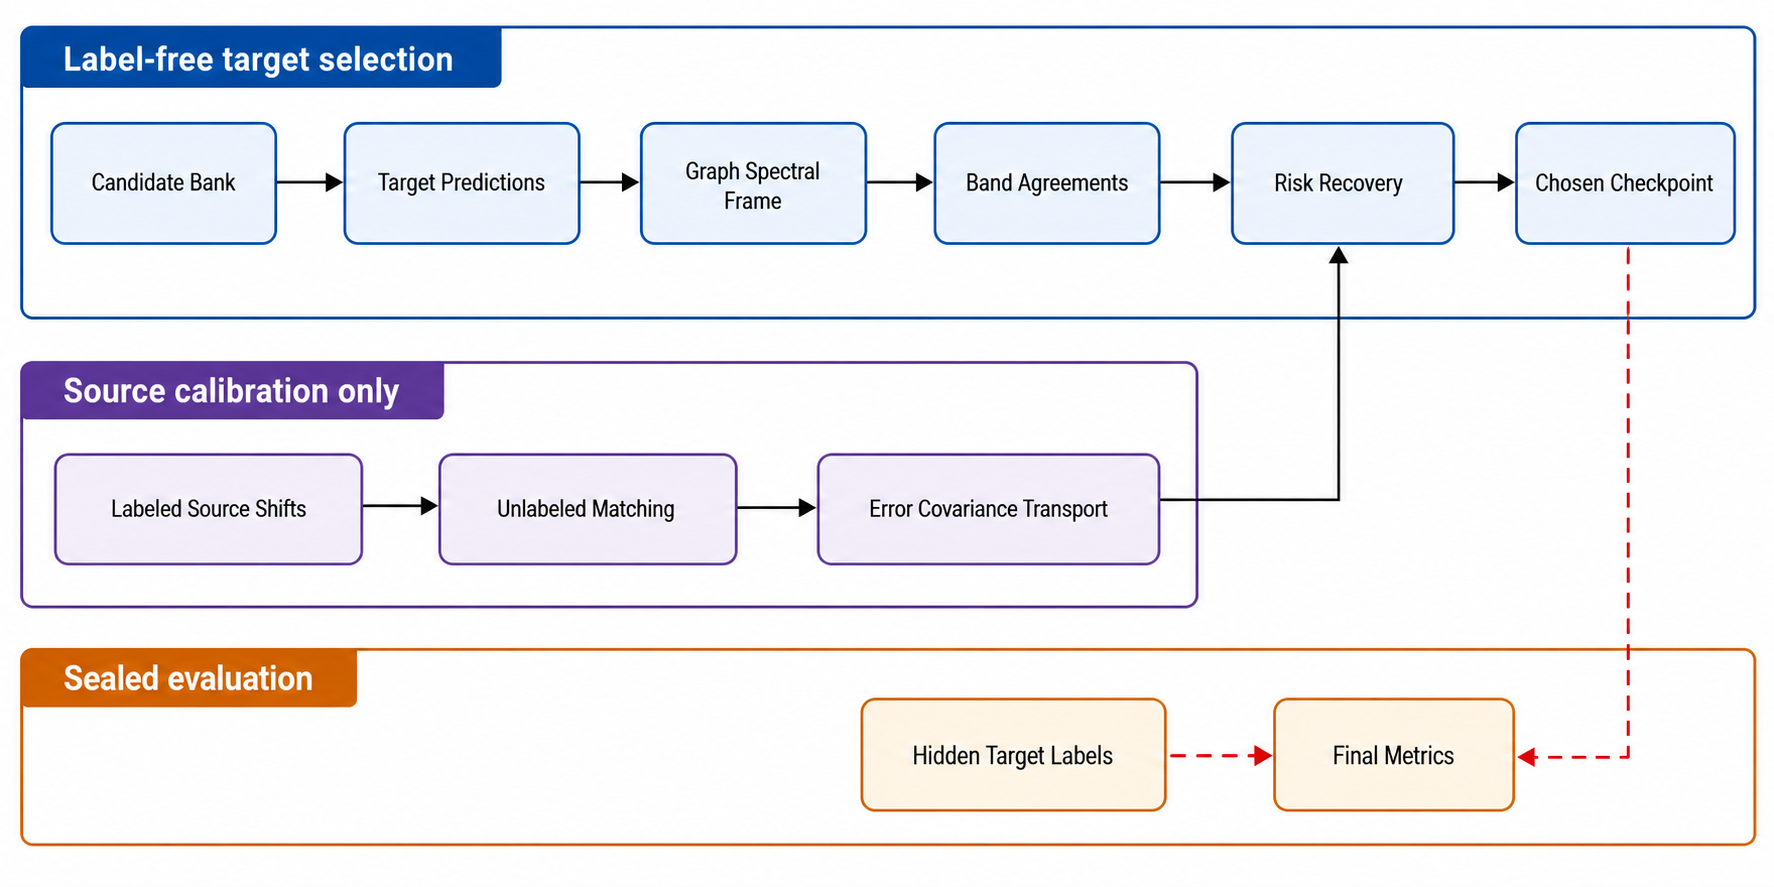
\includegraphics[width=0.96\textwidth]{figures/figure1-gpt-image-2.png}
  \caption{\textbf{\benchmark protocol and \method research module.} The
  selector sees a frozen candidate bank and unlabeled target predictions.
  \method combines graph-spectral disagreement with covariance estimated from
  labeled source simulations. Target labels remain isolated in the evaluator.
  Under the registered audit reported in this paper, no selector passed all
  promotion guards, so the final twelve sealed transfers were not queried.}
  \label{fig:pipeline}
\end{figure*}

The empirical study follows a pre-registered stopping rule. On 44
source-simulated folds, covariance correction is the dominant source of
recovery accuracy, whereas spectral conditioning contributes only a modest,
statistically inconclusive increment over global covariance. On four
real-target open-development tasks, Agreement top-$20\%$ followed by Transfer
Score is the strongest diagnostic pipeline, reducing mean normalized regret
from $0.216807$ to $0.087507$. However, this pipeline is not owned by
\method, remains non-inferior on only $2/4$ tasks, and exceeds the worst-task
threshold. Five subsequent structural iterations fail to repair these
weaknesses. The registered audit therefore stops development without freezing
a selector and leaves the final twelve transfers sealed.

Our contributions are threefold:
\begin{itemize}
  \item \textbf{An auditable selection benchmark.} \benchmark jointly evaluates
  algorithm, configuration, seed, and checkpoint selection under immutable
  candidate-bank hashes, sealed target labels, and explicit stopping rules.
  \item \textbf{Covariance-aware risk-recovery theory.} We derive an exact
  graph-spectral disagreement identity and recovery bounds that make
  cross-model error covariance, frame approximation, and covariance
  misspecification explicit.
  \item \textbf{A pre-registered negative audit with failure localization.}
  We document which plausible trust, trajectory, coverage, and stability
  mechanisms fail, and show that $79.5\%$ of the remaining regret arises from
  shortlist-internal reranking after the oracle trajectory is already covered.
\end{itemize}
